\section*{Exercício 2}
\label{ex:2}
\addcontentsline{toc}{section}{Exercício 2}

    \begin{enumerate}
        \item %Ax
            \begin{itemize}
            	\item Dada proposição $Z\{\sum_{i=0}^{n}x[i] \} = \frac{1}{1-z^{-1}}X(z)$, sua demonstração encontra-se abaixo.
            	
            	\begin{proof}
            	\begin{equation}
            	\begin{split}
            	Z\left\{\sum_{i=0}^{n}x[i] \right\} & = \sum_{n=0}^{\infty} z^{-n} \sum_{i=0}^{n} x[i] \\
            	& = x[0] + z^{-1} \sum_{i=0}^{1} x[i] + z^{-2} \sum_{i=0}^{2} x[i] + \cdots \\
            	& = x[0] \sum_{i=0}^{\infty} z^{-i} + x[1] \sum_{i=1}^{\infty} z^{-i} + \cdots + x[k] 
            	\underbrace{\sum_{i=k}^{\infty} z^{-i}}_{\frac{z^{-k}}{1 - z^{-1}}} + \cdots\\
            	& = x[0] \frac{1}{1 - z^{-1}} + x[1] \frac{z^{-1}}{1 - z^{-1}} + \cdots \\
            	& = \frac{1}{1 - z^{-1}} \underbrace{\sum_{i=0}^{\infty} x[i].z^{-i}}_{\coloneqq X(z)}
            	\end{split}
            	\end{equation}
            
            	\begin{equation}
            	\therefore Z\left\{\sum_{i=0}^{n}x[i] \right\} = \frac{1}{1-z^{-1}}.X(z) \hspace{10pt} \blacksquare
            	\end{equation}
            	\end{proof}
            	
            	\item De mesma forma, a demonstração da proposição $Z\{\sum_{i=0}^{n}x[i-1] \} = \frac{z^{-1}}{1-z^{-1}}X(z)$ encontra-se abaixo.
                
            	\begin{proof}
            	\begin{equation}
            	\begin{split}
            	Z\left\{\sum_{i=0}^{n}x[i] \right\} & = \sum_{n=0}^{\infty} z^{-n} \sum_{i=0}^{n} x[i-1] \\
            	& = x[-1] + z^{-1} \sum_{i=0}^{1} x[i-1] + z^{-2} \sum_{i=0}^{2} x[i-1] + \cdots \\
            	& = \underbrace{x[-1]}_{\coloneqq 0} \sum_{i=0}^{\infty} z^{-i} + x[0] \sum_{i=1}^{\infty} z^{-i} + \cdots \\
            	& = x[0] \frac{z^{-1}}{1 - z^{-1}} + x[1] \frac{z^{-2}}{1 - z^{-1}} + \cdots \\
            	& = \frac{z^{-1}}{1 - z^{-1}} \underbrace{\sum_{i=0}^{\infty} x[i].z^{-i}}_{\coloneqq X(z)}
            	\end{split}
            	\end{equation}
            
            	\begin{equation}
            	\therefore Z\left\{\sum_{i=0}^{n}x[i-1] \right\} = \frac{z^{-1}}{1-z^{-1}}.X(z) \hspace{10pt} \blacksquare
            	\end{equation}
                \end{proof}
                
            	\item Por fim, a proposição $\lim\limits_{z \rightarrow 1} X(z) = \sum_{i=0}^{\infty}x[i]$ segue
                
                \begin{proof}
            	\begin{equation}
            	\lim\limits_{z \rightarrow 1} X(z) = \lim\limits_{z \rightarrow 1} \sum_{i=0}^{\infty} x[i].z^{-i} = \sum_{i=0}^{\infty} x[i]
            	\end{equation}
            	
            	\begin{equation}
            	\begin{split}
            	\therefore \lim\limits_{z \rightarrow 1} X(z) = \sum_{i=0}^{\infty}x[i] \hspace{10pt} \blacksquare
            	\end{split}
            	\end{equation}
                \end{proof}
            	
            \end{itemize}
        
        \item\label{item:ex2b} %B
        
        Dada função $x_1(t) = \frac{1}{a} \left( 1 - e^{-at} \right)$, por definição, tem-se que:
        
        	\begin{equation}
            	\begin{split}
                	Z\{x_1(t)\} = X_1(z) & = \sum_{i=0}^{\infty} x_1(i Ts).z^{-i} \\
                	& = \frac{1}{a} \sum_{i=0}^{\infty} \left( 1 - e^{-a T_s i} \right)z^{-i} \\
                	& = \frac{1}{a} \sum_{i=0}^{\infty} z^{-i} - \frac{1}{a} \sum_{i=0}^{\infty} \underbrace{e^{-a T_s i}.z^{-i}}_{(z.e^{aT_s})^{-i}}
            	\end{split}
        	\end{equation}
        
        Se $|z| > 1$ e $|z| > e^{aT_s}$, então:
        	
        	\begin{equation}
            	\begin{split}
                	\frac{1}{a} \sum_{i=0}^{\infty} z^{-i} - \frac{1}{a} \sum_{i=0}^{\infty} e^{-a T_s i}.z^{-i} & = \frac{1}{a} (\frac{1}{1-z^ {-1}} - \frac{1}{1-e^{-aT_s} z^ {-1}}) \\
                	& = \frac{1}{a} \frac{(1 - e^{-aT_s})z^{-1}}{(1-z^{-1})(1-e^{-aT_s} z^ {-1})}
            	\end{split}
        	\end{equation}
        	
        Portanto
        	
        	\begin{equation}
            	X_1(z) = \frac{1}{a}  \frac{(1 - e^{-aT_s})z^{-1}}{(1-z^{-1})(1-e^{-aT_s} z^{-1})}
        	\end{equation}
        
        De mesma forma, dada função $x_2(t) = t^2 e^{-a t}$, por definição tem-se que:
        
        	\begin{equation}
            	\begin{split}
                	Z\{x_2(t)\} = X_2(z) & = \sum_{i=0}^{\infty} x_2(i Ts).z^{-i} \\
                	& = \sum_{i=0}^{\infty} \left( i^2 T_s^2 e^{-a T_s i} z^{-i} \right) \\
                	& = \sum_{i=0}^{\infty} T_s^2 i^2 e^{-a T_s i} z^{-i}
            	\end{split}
        	\end{equation}
        	
        Por meio da propriedade da transformada $\mathcal{Z}\{n X[n]\} \coloneqq -z \frac{d}{dz} X(z)$, segue
        
            \begin{subequations}
                \begin{equation}
                    x[n] = e^{-an} \rightarrow -z \frac{d}{dz} \mathcal{Z}\{e^{-an}\} = \mathcal{Z}\{n e^{-an}\} \mbox{, } n = T_s i \mbox{, } i \in \mathbb{N}
                \end{equation}
                \begin{equation}
                    x[n] = n e^{-an} \rightarrow -z \frac{d}{dz} \mathcal{Z}\{n e^{-an}\} = \mathcal{Z}\{n^2 e^{-an}\} \mbox{, } n = T_s i \mbox{, } i \in \mathbb{N}
                \end{equation}
            \end{subequations}
        
        Logo
        
            \begin{equation}
                \begin{split}
                    \mathcal{Z}\{e^{-an}\} & = \frac{1}{1 - e^{-a T_s} z^{-1}} \Rightarrow \\
                    \frac{d}{dz} \mathcal{Z}\{e^{-an}\} & = - e^{-a T_s} \frac{z^{-2}}{(1 - e^{-a T_s} z^{-1})^2} \\
                    \mathcal{Z}\{n e^{-an}\} \coloneqq -z \frac{d}{dz} \mathcal{Z}\{e^{-an}\} & = e^{-a T_s} \frac{z^{-1}}{(1 - e^{-a T_s} z^{-1})^2}
                \end{split}
            \end{equation}
        
        e
        
            \begin{equation}
                \begin{split}
                    \mathcal{Z}\{n e^{-an}\} & = e^{-a T_s} \frac{z^{-1}}{(1 - e^{-a T_s} z^{-1})^2} \Rightarrow \\ \frac{d}{dz} \mathcal{Z}\{n e^{-an}\} & = e^{- a T_s} \frac{z^{-2}(1 - e^{-a T_s} z^-1)^2 - 2(1 - e^{-a T_s} z^{-1}) e^{-a T_s} z^{-2}}{(1 - e^{-a T_s} z^{-1})^3} \\ 
                    & = - e^{-a T_s} \frac{z^{-2} (1 + e^{-a T_s} z^{-1})}{(1 - e^{- a T_s} z^-1)^3}
                \end{split}
            \end{equation}
        
        Portanto 
        
            \begin{equation}
                \mathcal{Z}\{n^2 e^{-a n}\} \coloneqq -z \frac{d}{dz} \mathcal{Z}\{n e^{-a n}\} = e^{-a T_s} \frac{z^{-1}(1 + e^{-a T_s} z^{-1})}{(1 - e^{-a T_s} z^{-1})}
            \end{equation}
        
        Em ambos os casos, a região de convergência é dada pela condição $R = R_1 \cap R_2$, com $R_1 = \left\{z \in \mathbb{C} | |z| \leq 1 \right\}$ e $R_2 = \left\{z \in \mathbb{C} | |z| \leq e^{-a T_s} \right\}$
        
        \item %C
        
        Por definição, a equação das diferenças é da forma
        
            \begin{equation}
                \sum_{i=0}^{m} b_i y[n-i] = \sum_{i=0}^{n} a_i x[n-i]
            \end{equation}
        
        A função de transferência equivalente é
        
            \begin{equation}
                G(z) = \frac{Y(Z)}{X(z)} = \frac{\sum_{i=0}^{m} b_{i} z^{-i}}{\sum_{i=0}^{n} a_{i} z^{-i}} = \frac{\sum_{i=0}^{m} b_{m-i} z^{i}}{\sum_{i=0}^{n} a_{n-i} z^{i}}
            \end{equation}
        
        Assim, com parâmetros dados por $m = n = 3$ e $a_i, b_i$, $i = 1, 2, 3$ dados por $a_0 = 1$, $a_1 = -0.9737$, $a_2 = 0.8101$, $a_3 = 0.8151$, $a_1 = -0.0515$, $b_0 = 0.4108$, $b_1 = -1.0094$, $b_2 = 1.0094$ e $b_3 = 0.4108$, as raízes do numerador e denominador, nomeadamente zeros e pólos, são respectivamente $z = \{1.38 \pm 1.18 i, -0.3\}$ e $p = \{0.45 \pm 0.74i, 0.068\}$.
        
        \item %D
        
            \begin{itemize}
                \item Para a série $x[n] = a^n u[n]$, sua transformada $\mathcal{Z}$ é:
                    \begin{equation}
                        \begin{split}
                            X(z) &= \sum_{n = -\infty}^{\infty} a^n u[n] z^{-n} \\
                            & = \sum_{n 
                            = 0}^{\infty} a^n z^{-n} = \sum_{n = 0}^{\infty} (\frac{a}{z})^n \stackrel{|z| > |a|}{=} \frac{1}{1 - \frac{a}{z}} \\
                            &= \frac{1}{1 - a z^{-1}} \\
                            \therefore & \,\, G(z) = \frac{1}{1 - a z^{-1}}
                        \end{split}
                    \label{eq:anun}
                    \end{equation}
                
                \item Para a série $x[n] = -a^n u[-n-1]$, sua transformada $\mathcal{Z}$ é:
                    \begin{equation}
                        \begin{split}
                            X(z) &= - \sum_{n = - \infty}^{\infty} a^n u[-n - 1] z^{-1} \\
                            &= - \sum_{n = -1}^{-\infty} a^n z^{-n} \\
                            &= -\left(a^{-1}z + a^{-2} z^2 + a^{-3} z^3 + \cdots\right) \\
                            &= -\frac{z}{a} \sum_{n = 0}^{\infty} (\frac{z}{a})^n \stackrel{|z| < |a|}{=} - \frac{z}{a} \frac{1}{1 - \frac{z}{a}} = \frac{z}{z-a} = \frac{1}{1 - a z^{-1}} \\
                            \therefore & \,\, G(z) = \frac{1}{1 - a z^{-1}} \\
                            \therefore G(z) = \frac{1}{1 - a z^{-1}}
                        \end{split}
                    \label{eq:_anun_1}
                    \end{equation}
            \end{itemize}
        \end{enumerate}
    
    Ambos os sinais apresentam a mesma transformada $\mathcal{Z}$, apesar de serem distintos. Entretanto, as regiões de convergência de ambos são distintas: para \eqref{eq:anun}, esta é  $|z| > |a|$ e para \eqref{eq:_anun_1}, $|z| < |a|$. A imagem \ref{fig:ex2d} apresenta as regiões visualmente.
    
    \begin{figure}[H]
        \centering
            \begin{tabular}{cc}
                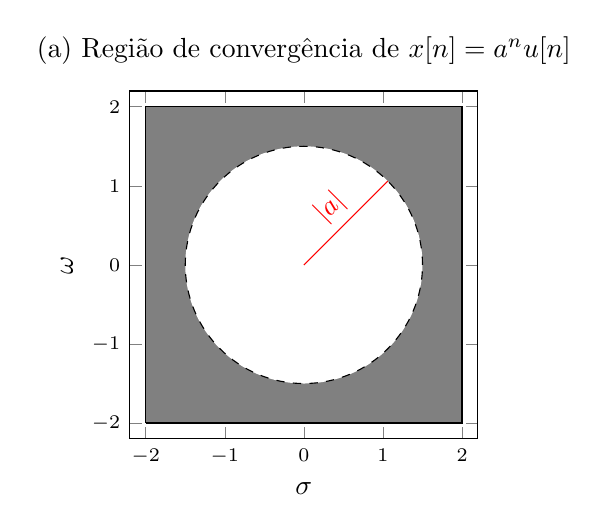
\begin{tikzpicture}
                    \begin{axis}[
                        title={(a) Região de convergência de $x[n] = a^n u[n]$},
                        width=6cm, height=6cm,
                        xmin=-2, xmax=2,
                        ymin=-2, ymax=2,
                        xlabel = {$ \sigma $}, ylabel = {$ \omega $},
                        xtick={-2, -1, 0, 1, 2},
                        xticklabels={$-2$, $-1$, $0$,$1$,$2$},
                        ytick={-2, -1, 0, 1, 2},
                        yticklabels={$-2$, $-1$, $0$,$1$,$2$},
                        every tick label/.append style={font=\scriptsize},
                        enlargelimits=0.05,
                        ]
                        
                        % Draw filled rectangle
                        \addplot[draw=black, fill=gray, thin] coordinates { (-2,-2) (-2, 2) (2, 2) (2, -2) (-2, -2) };
                        
                        % Draw filled circles
                        \draw[black, dashed, fill = white] (axis cs:0, 0) circle[radius=1.5];
                        
                        % Draw diameter
                        \addplot[color=red] coordinates { (1.5/1.4142, 1.5/1.4142) (0, 0) } node[pos=.5, yshift=8pt,sloped] {$|a|$};
                    
                    \end{axis}
                \end{tikzpicture} &
                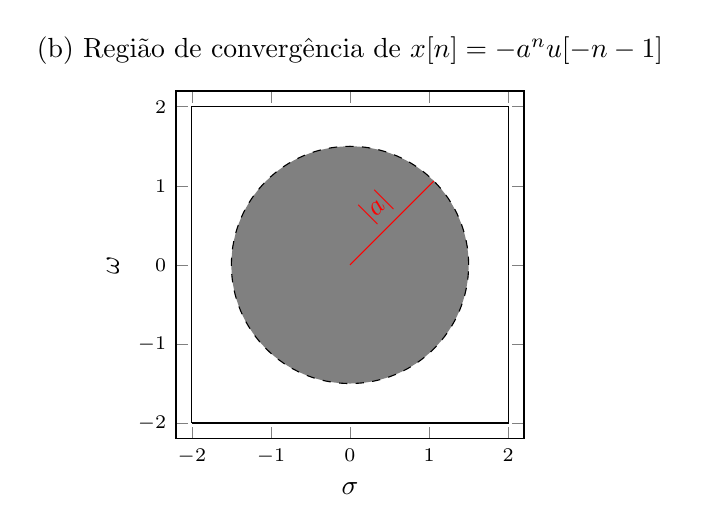
\begin{tikzpicture}
                        \begin{axis}[
                            title={(b) Região de convergência de $x[n] = -a^n u[-n-1]$},
                            width=6cm, height=6cm,
                            xmin=-2, xmax=2,
                            ymin=-2, ymax=2,
                            xlabel = {$ \sigma $}, ylabel = {$ \omega $},
                            xtick={-2, -1, 0, 1, 2},
                            xticklabels={$-2$, $-1$, $0$,$1$,$2$},
                            ytick={-2, -1, 0, 1, 2},
                            yticklabels={$-2$, $-1$, $0$,$1$,$2$},
                            every tick label/.append style={font=\scriptsize},
                            enlargelimits=0.05,
                            ]
                            
                            % Draw filled rectangle
                            \addplot[draw=black, fill=white, thin] coordinates { (-2,-2) (-2, 2) (2, 2) (2, -2) (-2, -2) };
                            
                            % Draw filled circles
                            \draw[black, dashed, fill = gray] (axis cs:0, 0) circle[radius=1.5];
                            
                            % Draw diameter
                            \addplot[color=red] coordinates { (1.5/1.4142, 1.5/1.4142) (0, 0) } node[pos=.5, yshift=8pt, sloped] {$|a|$};
                        
                        \end{axis}
                \end{tikzpicture}
            \end{tabular}
        \caption{\label{fig:ex2d} Região de convergência da transformada $\mathcal{Z}$ das sequências $x[n] = a^n u[n]$ e $x[n] = -a^n u[-n-1]$}
    \end{figure}

